\documentclass[a4paper,12pt,fleqn]{article}%fleqn pour aligner les equations à gauche
\usepackage{graphicx}
\usepackage[utf8]{inputenc}  
\usepackage[T1]{fontenc}
\usepackage{lscape}

\usepackage{tgheros,textcomp}%Police Arial
\renewcommand{\familydefault}{\sfdefault}

%\setlength{\mathindent}{0pt}%indentation dans math = 0

\usepackage[top = 1cm, bottom = 2cm, left = 1cm, right = 1cm]{geometry}
\usepackage{titlesec}
%\setcounter{secnumdepth}{4}
\usepackage{xcolor}
\usepackage{amssymb} %double flèche de réaction
\usepackage{mathrsfs}%farraday
\usepackage{xtab}%tableau sur plusieurs pages
\usepackage{esvect}%grands vecteurs

\usepackage[version=4]{mhchem} %equations chimiques

\usepackage{array}
\usepackage{chemfig}
\usepackage{multirow}
%\usepackage{sectsty}

\usepackage{caption}
\usepackage{adjustbox}
\usepackage[labelformat=simple]{subfig}
\usepackage{float}


\usepackage{amsmath}
\usepackage{amssymb}
\usepackage[cal=boondoxo]{mathalfa} 
\usepackage{enumitem}
\usepackage{lastpage}
\usepackage{tcolorbox}
\usepackage{siunitx}
\usepackage[european, straightvoltages, RPvoltages]{circuitikz}
\usepackage{tikz}
\usetikzlibrary{shapes.geometric}
\usetikzlibrary{calc}
\usetikzlibrary{automata,positioning}
\usepackage{multicol}
\usepackage{eqnarray}
\usepackage{tabularx,colortbl}%colorer fond cellules

\sisetup{
	detect-all,
	output-decimal-marker={,},
	group-minimum-digits = 3,
	group-separator={~},
	number-unit-separator={~},
	inter-unit-product={~}
} %setup pour SIunitx

\usepackage{listings}%pour insérer le code python
\definecolor{codegreen}{rgb}{0,0.6,0}
\definecolor{codegray}{rgb}{0.5,0.5,0.5}
\definecolor{codepurple}{rgb}{0.58,0,0.82}
\definecolor{backcolour}{rgb}{0.95,0.95,0.92}


\titleformat{\section}
{\titlerule
\vspace{.8ex}%
\normalfont \bfseries}
{\thesection :}{.5em}{\bfseries}

\renewcommand{\thesection}{Exercice \arabic{section}}
\titlespacing{\section}{0pt}{1em}{1em}
\renewcommand{\thesubsection}{\hspace{1cm}\alph{subsection}.}
\renewcommand\thesubfigure{\textbf{Document \arabic{subfigure} :}}

\title{\vspace{-1cm}\large 
	\begin{tabular}{|>{\centering}m{5cm}|>{\centering}m{8cm}|>{\centering\arraybackslash}m{4cm}|}
		\hline
		Exercices & \textbf{\textsc{Mouvement}} &  Chapitre 6 \\
		\hline
\end{tabular}}
\date{}

\newpagestyle{mystyle}{%
	\setfoot{ROSALIE}{\thepage\,$|$\,\pageref{LastPage}}{}
}
\renewpagestyle{plain}{%
	\setfoot{ROSALIE}{\thepage\,$|$\,\pageref{LastPage}}{}
}

\pagestyle{mystyle}

\newenvironment{itemize*}%
{\begin{itemize}[label=$-$]%
		\setlength{\itemsep}{0pt}%
		\setlength{\parskip}{0pt}}%
	{\end{itemize}}

\newenvironment{itemize**}%
{\begin{itemize}[label=,labelindent=0pt, leftmargin=*,topsep=0pt]%
		\setlength{\itemsep}{0pt}%
		\setlength{\parskip}{0pt}}%
	{\end{itemize}}

\renewcommand{\arraystretch}{1.5}

  
  
\begin{document}
\maketitle
\vspace{-2.5cm}
\begin{multicols}{2}
\section{La grêle}
La grêle peut avoir des effets dévastateurs pour les habitants et les agriculteurs en raison de la vitesse que les grêlons acquièrent lors de leur chute. En effet, le grêlon chute avec une vitesse initiale nulle puis accélère jusqu'à atteindre une vitesse limite de \SI{70}{\kilo\meter\per\hour}.
\begin{enumerate}
	\item Définir le système et le référentiel d'étude.
	\item Le système est assimilé à un point matériel. Quel(s) aspect(s) ne peut-on pas aborder lors de cette étude ?
	\item Comment évolue le vecteur vitesse lors de la première phase de la chute ?
	\item Donner la direction, le sens et la norme du vecteur en \unit{\meter\per\second} lors de la deuxième phase de la chute.
	\item Comment qualifier le mouvement durant cette deuxième phase ?
\end{enumerate}

\section{Mobile autoporteur}
Dans le référentiel terrestre, un mobile autoporteur, placé sur une table parfaitement horizontale, est attaché par un fil à un point fixe noté $O$. On rappelle qu'un mobile autoporteur évolue sur un coussin d'air supprimant les frottements et est muni d'un dispositif qui produit des marques à intervalles de temps réguliers (ici $\Delta t = \SI{40}{ms}$) ce qui permet de repérer les positions de son centre d'inertie sur une feuille de papier. Les points où la feuille se papier a été localement marquée sont repérés par des petites croix.
\begin{enumerate}
    \item Quelles est la nature de la trajectoire du centre d'inertie du mobile autoporteur ?
    \item Déterminer l'échelle spatiale du document.
    \item Calculer la valeur de la vitesse instantanée aux points $G_2$, $G_3$, $G_4$ et $G_5$.
    \item Représenter les vecteurs vitesse en ces points avec l'échelle \SI{1,0}{cm} pour \SI{0,25}{\meter\per\second}, en rouge.
    \item En se basant sur les vecteurs tracés, décrire la nature du mouvement.
\end{enumerate}
\begin{figure}[H]
    \centering
    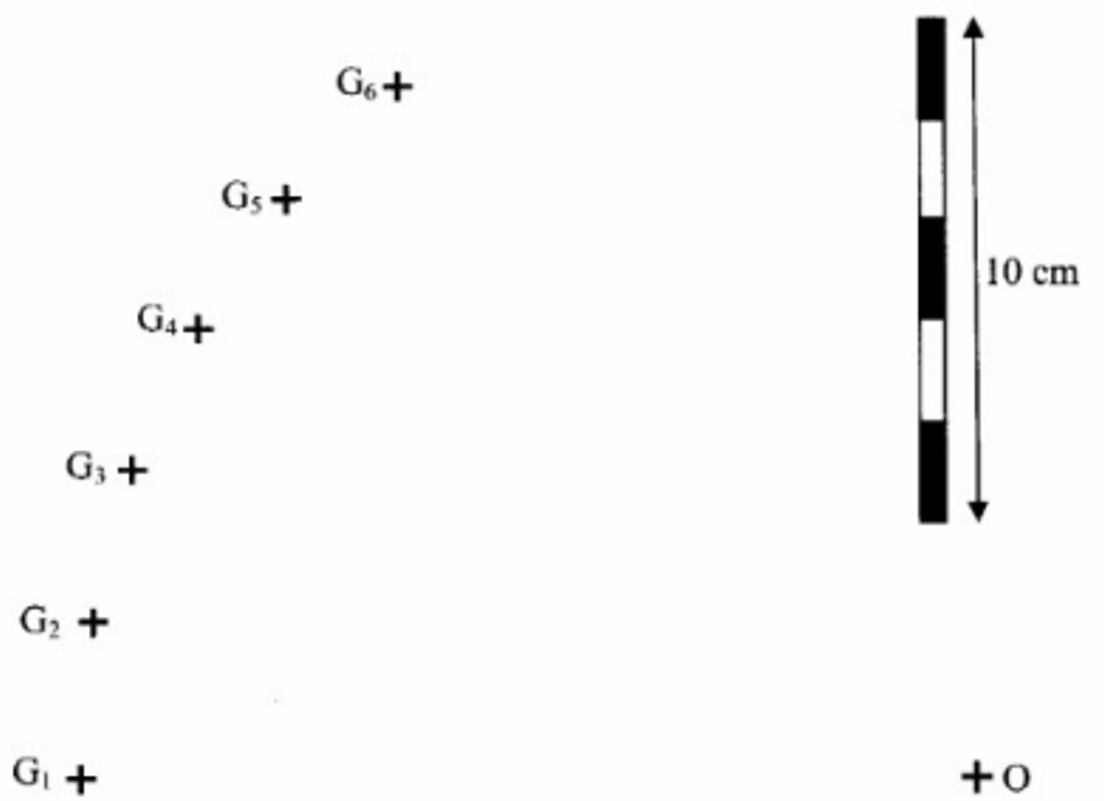
\includegraphics[width=\linewidth]{Ressources/2GT_C6_Exercices2_Fig1.png}
\end{figure}
\section{Station spatiale internationale}
La station spatiale internationale (ISS) est une station spatiale en orbite circulaire basse autour de la Terre. Des astronautes internationaux y mènent des expériences de recherche scientifique en milieu spatial. Située à une altitude d'environ 330 km, l'ISS effectue un tour complet en 93 minutes.
\begin{enumerate}
	\item Quel est le référentiel adapté à l’étude du mouvement de l’ISS ?
	\item Décrire le mouvement de l’ISS dans ce référentiel.
	\item Calculer la valeur de la vitesse de la station.
	\item Décrire la variation de son vecteur vitesse.
	\item Combien de tours effectue l’ISS en une journée ?
\end{enumerate}

\textbf{Donnée :} Rayon de la Terre $R_T$ = \SI{6370}{km}
\end{multicols}
\end{document}